\chapter{Funktio}

Usein ollaan kiinnostuneita siitä, millainen yhteys kahden asian välillä
on. Funktio on matemaattinen työkalu näiden yhteyksien tarkastelemiseen.

\laatikko{
\emph{Funktio} $f(x)$ liittää \emph{muuttujaan} $x$ arvon $f(x)$.

Funktiolla on \emph{määrittelyjoukko} $A$, johon muuttuja $x$ kuuluu, ja \emph{arvojoukko} $B$, johon funktion arvot kuuluvat.
}

\begin{esimerkki}
Hyödykkeen ja siitä maksettavan arvonlisäveron välistä yhteyttä
voidaan kuvata funktiolla. Valitaan funktion määrittelyjoukoksi
tavaroiden joukko,
\[
A = \{\text{ahvenfilee}, \text{AIV-rehu}, \text{auto}, \text{runokirja}, \text{ravintola-ateria}, \text{särkylääke}, \text{televisio}\},
\]
ja arvojoukoksi reaaliluvut. Funktio liittää kuhunkin määrittelyjoukon
hyödykkeeseen siitä maksettavan arvonlisäveroprosentin: esimerkiksi
$f(\text{särkylääke}) = 9$ ja $f(\text{televisio}) = 23$.

\begin{center}
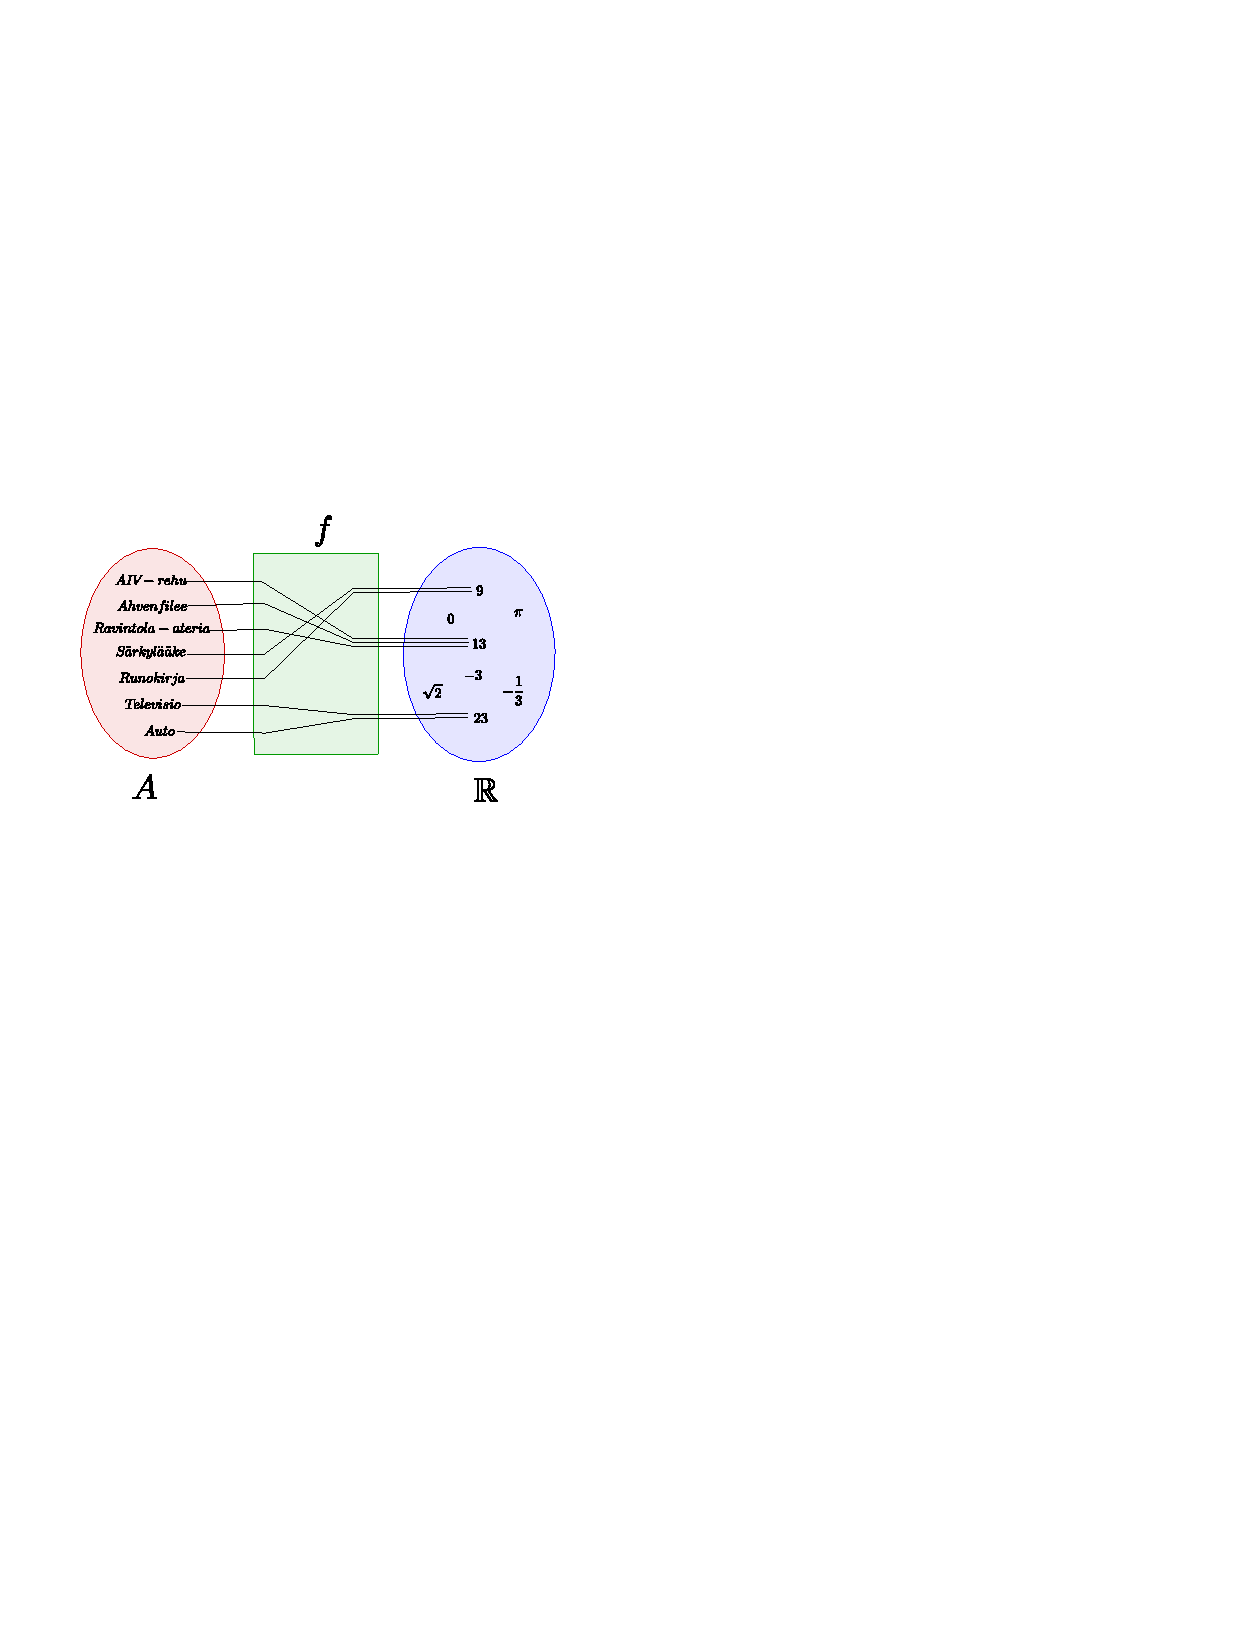
\includegraphics[width=13cm]{03-funktiot/kuvia/funktiokone.pdf}
\end{center}
\end{esimerkki}


Funktioihin liittyy monia vakiintuneita käytäntöjä, esimerkkinä seuraavat:
\begin{itemize}
\item $f(x) = y$ lausutaan: ''Funktio saa arvon $y$ pisteessä $x$'',
\item Funktion määrittely- ja maalijoukot jätetään usein merkitsemättä, jos ne ovat selviä asiayhteydestä. Tällä kurssilla maalijoukko on yleensä reaaliluvut.
\item Funktion sääntöä kutsutaan usein pelkästään funktioksi.
\item Toisinaan funktion säännölle ja funktion kuvaajalle ei tehdä selkeää eroa:
$y = f(x)$ samaistetaan koordinaatistoon piirretyn funktion kuvaajan kanssa.
\end{itemize}

Funktion sääntö voidaan usein kirjoittaa matemaattisena kaavana.


\begin{esimerkki}
Jos neliön sivun pituutta merkitään $x$:llä, voidaan sivun pituuden
ja neliön pinta-alan välistä yhteyttä kuvata funktiolla
$A = f(x) = x^2$.
\end{esimerkki}

Funktion \emph{arvojoukko} koostuu niistä maalijoukon alkioista,
jotka funktio saa arvokseen ainakin yhdessä määrittelyjoukon pisteessä.

%\esimerkki{Määritellään funktio $f$ kaavalla
\[f(x) = \frac{1}{x-1}.\]. Mitkä ovat funktion
\begin{enumerate}[a)]
 \item määrittelyjoukko,
 \item arvojoukko?
\end{enumerate}

\textbf{Ratkaisu.}
\begin{enumerate}[a)]
\item Funktion määrittelyn yhteydessä ei ole kerrottu funktion määrittelyjoukkoa,
joten se täytyy päätellä asiayhteydestä.

Havaitaan, että funktion $f(x)$ arvo voidaan laskea kaikilla $x$:n
arvoilla lukuun ottamatta arvoa $x = 1$. Yleensä funktion määrittelyjoukoksi
oletetaan laajin joukko, jolla funktion arvo voidaan laskea.

\item Funktion arvojoukko koostuu niistä luvuista, jotka funktio
saavuttaa muuttujan $x$ eri arvoilla. Arvojoukon selvittämiseksi
tutkitaan, millä vakion $a$ arvoilla yhtälöllä $f(x) = a$ on
ratkaisu,
\begin{align*}
a &= \frac{1}{x-1} & &| \, \text{Oletetaan, että $x \neq 1$, jolloin voimme kertoa $(x-1)$:llä puolittain.} \\
a(x-1) &= 1 \\
x-1 &= \frac{1}{a} \\
x &= 1+\frac{1}{a} & &| \, \text{Havaitaan, että yhtälöllä on ratkaisu
kaikilla $a \neq 0$.}
\end{align*}
\end{enumerate}
}
